\documentclass{article}

\usepackage[utf8]{inputenc}
\usepackage[spanish]{babel}
\usepackage{fullpage}
\usepackage{hyperref}
\usepackage{graphicx}



\title{Informe de tesis de licenciatura}
\author{Ionatan Perez}
\date{\today}

\begin{document}

\maketitle

\section{Introducción}

    Los mecanismos y dispositivos de sustitución sensorial (SSD) son técnicas en las cuales los estimulo generados en nuestro entorno y que normalmente son percibido a través de un dado sentido son reemplazados por otro estimulo (pero que codifica información equivalente) de manera que pueda ser percibido a través de un sentido sensorial alternativo. Típicamente estas técnicas son utilizadas por personas que carecen de alguno de los sentidos para poder percibir lo que de otra manera no podrían. Ejemplos cotidianos de estas técnicas son por ejemplo el bastón que suelen usar las personas ciegas, las marcas y guías en baldosas, el código braille, los timbres que encienden luces, las escalas cromáticas aptas para daltónicos, etc. 
    
    En particular, dentro de los problemas biológicos de percepción, el problema de la ceguera es un problema que conlleva limitaciones muy importantes para las personas que la sufren y que afecta a cerca de diez millones de personas en el mundo \cite{NroCiegos}. Como paliativo a dicha situación existen diferentes técnicas (algunas de muy baja complejidad, pero funcionalidad limitada) para sustituir sensorialmente los estímulos, como puede ser un bastón que al tacto permita reconocer obstáculos. Otras técnicas, mucho mas complejas y en actual desarrollo, apuntan a restituir la capacidad de visión mediante implantes que estimulen artificialmente al sistema nervioso\cite{Implantes1,Implantes2}, pero actualmente se encuentran en un estado muy temprano de desarrollo, solo sirven en casos específicos, poseen poca resolución y son muy invasivas \cite{Implantes3,Implantes4}. 
    
    Alternativamente a las técnicas que buscan restituir la visión en personas ciegas, están las técnicas que sustituyen los estímulos, estos estímulos pueden ser reemplazados por estímulos táctiles o bien auditivos. La representación táctil de los estímulos visuales comparte la propiedad intrínseca de ser percibida en un sistema de coordenadas bidimencional (la piel y la retina ambos poseen sensores distribuidos en una superficie). Los trabajos pioneros en este técnica fueron realizados por Paul Bach-y-Rita \cite{Tactil1} quien diseñó un dispositivo que sujeto en la espalda de las personas podía reproducir imágenes filmadas por una cámara. Sin embargo la baja resolución de este dispositivo (20x20 pixeles), junto a su tamaño hicieron que sea poco practico. En posteriores trabajos \cite{Tactil2} se reemplazó el dispositivo por uno colocado en la legua (que posee una sensibilidad muy alta) donde además se reemplazó el mecanismo de estímulo por uno de pequeñas descargas eléctricas. Este trabajo solucionó en buena parte el problema de la portabilidad del dispositivo (que media 3cmx3cm con 12x12 pixeles), pero sin embargo su capacidad de distinguir objetos sigue siendo reducida \cite{Tactil3}, comparable (sin entrenamiento) a 20/860 \footnote{Esta manera de indicar la capacidad visual de una persona representa cuan lejos tiene que estar (medido en pies si el numerador es 20) de dos puntos para distinguirlos en relación a una persona con visión plena. Se suele considerar a una persona con problemas de ceguera cuando su capacidad esta por debajo de 20/200}. Estudios \cite{Tactil4} muestran que con entrenamiento los sujetos pueden mejorar en cu capacidad de percepción, sin embargo hay una limitación básica en la resolución que permite este dispositivos que esta dado por la separación espacial de los electrodos y la capacidad de la lengua de distinguirlos. 
    
    \begin{figure}
        \center
        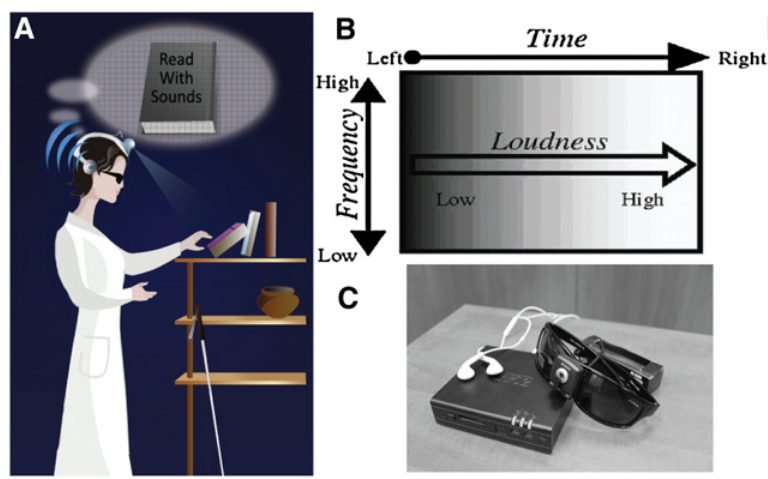
\includegraphics[width=0.8\textwidth]{Imagenes/Voice2.png}
        \caption{Dispositivo de sustitución sensorial vOICe y ejemplo de representación de las imagenes a través de dicho dispositivo.}
        \label{fig:Voice2}
    \end{figure}
    
    \begin{figure}
        \center
        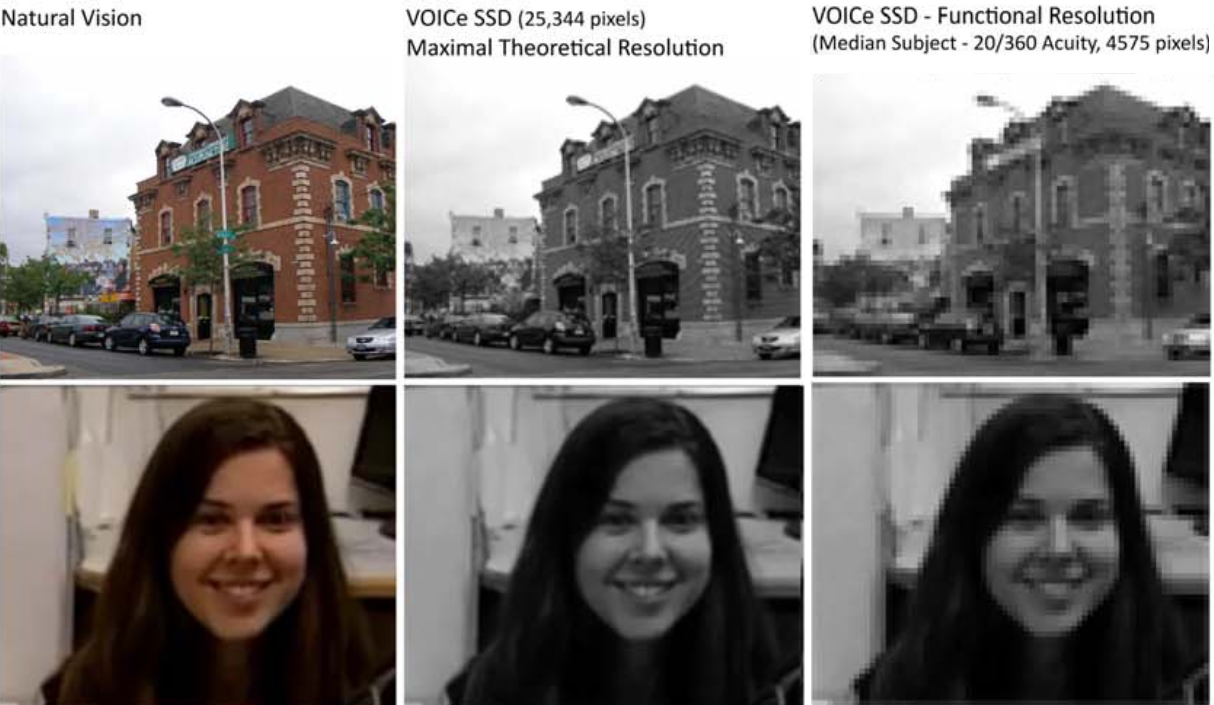
\includegraphics[width=0.8\textwidth]{Imagenes/ImagenVoice1.png}
        \caption{Perdida de resolución al utilizar una tecnología tipo vOICe, se compara la imagen original con la imagen pixelada luego del procesamiento y la resolución real observada en sujetos. \url{http://dx.doi.org/10.1371/journal.pone.0033136}}
        \label{fig:Voice1}
    \end{figure}
    
    \begin{figure}
        \center
        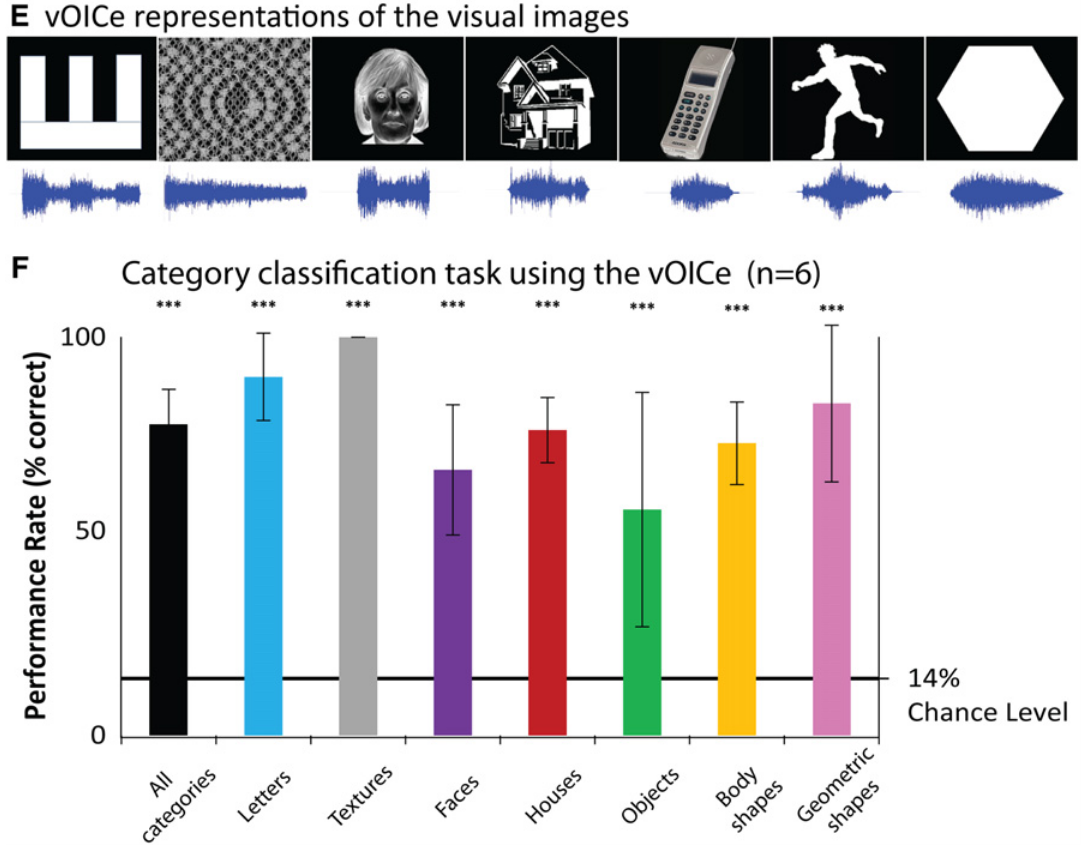
\includegraphics[width=0.7\textwidth]{Imagenes/Voice3.png}
        \caption{Ejemplo del sonido correspondiente a imágenes pertenecientes a diferentes categorías y la capacidad del distinguirlas en sujetos que fueron entrenados durante periodos de tiempo prolongado en la tecnología vOICe. \url{http://dx.doi.org/10.1016/j.neuron.2012.08.026}}
        \label{fig:Voice3}
    \end{figure}
    
    
    El otro mecanismo por el cual se puede realizar sustitución sensorial es transformando el estimulo visual en un estímulo sonoro. El primer prototipo de esta tecnología (denominada vOICe) fue desarrollado en 1992 \cite{Voice1} como un dispositivo portátil, de bajo costo y de resolución mayor a las alcanzadas por los métodos de sustitución táctil (ver figura \ref{fig:Voice1}). Con el tiempo se fueron desarrollando versiones mejores, de mayor resolución y adaptadas a las tecnologías mas modernas (ver figura \ref{fig:Voice2}).
    
    La tecnología vOICe (\url{https://www.seeingwithsound.com/}), a diferencia de la sustitución sensorial táctil presenta la libertad de elegir que parámetros del sonido se eligen para representar los parámetros que usualmente se observan con la vista. A priori hay una amplia libertad en la representación si utilizan efectos sonoros complejos, sin embargo, recurriendo a las características básica del sonido hay tres grados de libertad a la hora de crear un sonido: el tono o frecuencia, el volumen y la duración. Estas tres características son las que utiliza el vOICe para representar la información visual (codificada en escala de grises). El vOICe toma una imagen, la pixela, y representa la coordenada vertical de cada pixel en la frecuencia, la coordenada horizontal en el tiempo (o duración del pixel) y la intensidad (o brillo) del pixel en el volumen o intensidad del sonido. En otras palabras lo que hace es interpretar cada columna de la imagen como una antitransformada de fourier del sonido a generar. 
    
    A partir de esta concepción de sustitución sensorial, el vOICe se fue desarrollando sobre diferentes plataformas tecnológicas siendo hoy una aplicación disponible en diversas plataformas, incluyendo PCs, celulares, y otros dispositivos que sean capaces de grabar imágenes y reproducir sonidos. Además cuenta con herramientas integradas de utilidad para personas ciegas como ser comandos por vos, filtros del la imagen a procesar por color, geolocalizacion, etc. La version para celulares pude consultarse en \url{https://play.google.com/store/apps/details?id=vOICe.vOICe} y un manual para realizar el entrenamiento adecuado para su uso en \url {https://www.seeingwithsound.com/manual/The_vOICe_Training_Manual.htm} 
    
    En paralelo al desarrollo de la tecnología vOICe como aplicación, se realizaron otras pruebas e investigaciones, algunas sobre variantes en la representación sonora, como ser el caso de la denominada PSVA \cite{VoiceVariante1} que difiere del vOICe en que la escala vertical esta discretizada no en función de la resolución como numero de pixeles, sino respetando saltos que difieran en notas fijas, además posee una región de mayor resolución en la zona central de la imagen, simulando el funcionamiento del ojo. Otra variante es el denominado SmartSight que filtra y agrupa secciones de la imagen antes de realizar una representación sonora en forma de notas musicales \cite{VoiceVariantes2, VoiceVariantes3}. También sobre la base de codificar diferentes aspectos en términos de propiedades sonoras mas complejas, se esta desarrollando una versión similar el vOICe denominada EyeMusic que codifica en términos de notas la altura de los pixeles, pero utilizando diferentes instrumentos para representar diferentes colores \cite{VoiceVariantes4}.
    
    Por otro lado a partir del imágenes y mediciones de actividad cerebral y de entrenamiento se han realizado estudios acerca del funcionamiento subyacente al mecanismo de sustitución sensorial. Hay estudios que muestran que en el caso de personas ciegas de nacimiento se activas zonas típicas de procesamiento de la información para el canal sensorial utilizado, mientras que en personas que perdieron la visión siendo adultos se activan zonas del procesamiento de imágenes (frente a un mismo estimulo), o que la modulación de la actividad cerebral difiere entre personas que perdieron la vista a edad temprana y personas que simplemente reciben el estimulo con la vista tapada \cite{VoiceSubyacente1,VoiceSubyacente3}. También hay estudios que muestran que con entrenamiento los sujetos aprenden a reconocer patrones fijos e incluso pueden transferir el aprendizaje entre figuras similares \cite{VoiceSubyacente2}. Por otro lado estudios sobre la tecnología vOICe muestran que los sujetos son capaces de entrenar e integrar la percepción en tareas de reconocimiento de geometría espacial, siendo capaces de ubicar y señalar posicionamiento de objetos en un entorno 3D donde pueden cambiar el punto de vista de la cámara con la que observan los estímulos \cite{VoiceSubyacente4}
    
    Los trabajos previos sobre la tecnología vOICe muestran que los sujetos entrenados (que pueden ser tanto ciegos como videntes\cite{VoiceEntrenamiento1}) pueden aprender a distinguir entre categorías imágenes complejas \cite{VoiceEntrenamiento2} (como los que se observan en la figura \ref{fig:Voice3}), nosotros en nuestro trabajo intentamos sobre la base de un sistema de representación equivalente estudiar la capacidad no de interpretar figuras complejas, sino sencillas, pero en términos de categorías geométricas. 
    
    La idea detrás de la propuesta fue que, si bien a la hora de interactuar con entornos complejos es importante que el sistema de sustitución sensorial permita representar de forma equivalente información compleja, muchas actividades no requieren interactuar con estímulos complejos. Muchas veces los estímulos o bien son intrínsecamente sencillos (por ejemplo los iconos y contornos en la navegación dentro de una computadora) o bien se puede preprocesar la imagen para extraer con algoritmos las información mas relevante antes de realizar la sustitución sensorial. Por otro lado, estudiar la capacidad de detectar conceptos geométricos abstractos podría permitir inspeccionar, dentro de la compleja tarea de reconocer patrones, saber que aspectos son mas difíciles de identificar, cuales mas fáciles, y de que depende la dificultad a la hora de interpretar los sonidos. 
    
    Con ese objetivo en mente fue que nos propusimos realizar experimentos en los cuales se presentara a sujetos videntes estímulos sonoros codificados según la lógica del vOICe en pos de observar cual era la capacidad de los sujetos de distinguir los aspectos geométricos en estos estímulos. 


\section{Desarrollo Metodológico}

    Poder realizar los experimentos propuestos conllevo una larga lista de desafíos, elecciones y problemas técnicos a resolver, en muchos casos interrelacionados y desconociendo la dificultad que representaría cada elección a priori. Cualquiera de los diseños experimentales que nos propusiéramos tenía que consistir en la presentación de estímulos sonoros al usuario (o sujeto experimental) que debían ser respondido con alguna elección. Posteriormente correlacionando los estímulos presentados con las respuestas se podría evaluar la capacidad de percepción del sujeto. Pero la elección de estímulos, la secuencia en la cual presentarlos, el modo en que interactuaría el sujeto con el experimento, las condiciones de contorno en que sería realizado, y las preguntas especificas que buscábamos responder eran en un principio cuestiones abiertas.
    
    Algunas cuestiones que si estaban definidas eran que en un principio todos los sujetos serian videntes porque experimentos previos de entrenamiento \cite{VoiceEntrenamiento3} indicaban que los videntes presentan capacidades similares de aprender la representación que las personas ciegas, y conseguir sujetos tanto como interactuar con ellos durante el procedimiento experimental es muchísimo más fácil si los sujetos son videntes. Eventualmente una vez obtenidos resultados se podrían contrastar y validar en personas no videntes. 
    
    Por otro lado el experimento requeriría algún tipo de software que mostrara los estímulos y registrara las respuestas. Ese software tenía que ser desarrollado, y para evitar limitaciones a la hora de tomar futuras decisiones elegimos desarrollar la aplicación y toda la programación en LibGDX que es un framework de java que permite compilar a java para ejecutar el experimento en un entorno controlado de laboratorio; a java para android para realizar experimentos menos controlados pero más masivos; o a javascript para HTML5 con la idea de realizar experimentos a distancia. La elección del entorno de programación que daba mucha flexibilidad a la hora de diseñar el procedimiento experimental en función de los resultados iniciales tenia como contrapartida ciertas limitaciones a la hora de usar librerias y paquetes prearmados lo que implico finalmente un mayor trabajo de adaptación y programación para realizar tareas que en un entorno mas especifico quizas ya estaban resueltas. 
    
    
    

\clearpage


\begin{thebibliography}{9}

\bibitem{NroCiegos}
  WHO (2011) Fact Sheet Nu282
\bibitem{Implantes1}
Dowling J (2008) Current and future prospects for optoelectronic retinal prostheses. Eye 23: 1999–2005.
\bibitem{Implantes2}
Weiland JD, Cho AK, Humayun MS (2011) Retinal prostheses: current clinical results and future needs. Ophthalmology 118: 2227–2237.
\bibitem{Implantes3}
E Striem-Amit, A Bubic, A Amedi - 2012: Neurophysiological Mechanisms Underlying Plastic Changes and Rehabilitation following Sensory Loss in Blindness and Deafness
\bibitem{Implantes4}
Zrenner E, Bartz-Schmidt KU, Benav H, Besch D, Bruckmann A, et al. (2010) Subretinal electronic chips allow blind patients to read letters and combine them to words. Proceedings of the Royal Society B: Biological Sciences 278: 1489–1497.
\bibitem{Tactil1}
Bach-Y-Rita P, Collins C.C, Saunders F.A, White B, Scadden L. Vision substitution by tactile image projection. Nature. 1969;221:963–964. 
\bibitem{Tactil2}
Bach-Y-Rita P, Kaczmarek K.A, Tyler M.E, Garcia-Lara J. Form perception with a 49-point electrotactile stimulus array on the tongue: A technical note. J Rehabil Res Dev. 1998;35:427–430.
\bibitem{Tactil3}
Sampaio E, Maris S, Bach-Y-Rita P. Brain plasticity: ‘Visual’ acuity of blind persons via the tongue. Brain Res. 2001;908:204–207. 
\bibitem{Tactil4}
Chebat D.R, Rainville C, Kupers R, Ptito M. Tactile-‘visual’ acuity of the tongue in early blind individuals. Neuroreport. 2007;18:1901–1904
\bibitem{Voice1}
Meijer P.B. An experimental system for auditory image representations. IEEE Trans Biomed Eng. 1992;39:112–121.
\bibitem{VoiceVariante1}
Capelle C, Trullemans C, Arno P, Veraart C. A real-time experimental prototype for enhancement of vision rehabilitation using auditory substitution. IEEE Trans Biomed Eng. 1998;45:1279–1293. 
\bibitem{VoiceVariantes2}
Cronly-Dillon J, Persaud K, Gregory R.P. The perception of visual images encoded in musical form: A study in cross-modality information transfer. Proc Biol Sci. 1999;266:2427–2433. 
\bibitem{VoiceVariantes3}
Cronly-Dillon J, Persaud K.C, Blore R. Blind subjects construct conscious mental images of visual scenes encoded in musical form. Proc Biol Sci. 2000;267:2231–2238.
\bibitem{VoiceVariantes4}
Abboud, Sami, et al. "EyeMusic: Introducing a “visual” colorful experience for the blind using auditory sensory substitution." Restorative neurology and neuroscience 32.2 (2014): 247-257.
\bibitem{VoiceSubyacente1}
Poirier, Colline, Anne G. De Volder, and Christian Scheiber. "What neuroimaging tells us about sensory substitution." Neuroscience and Biobehavioral Reviews 31.7 (2007): 1064-1070.
\bibitem{VoiceSubyacente2}
Arno P, Capelle C, Wanet-Defalque M.C, Catalan-Ahumada M, Veraart C. Auditory coding of visual patterns for the blind. Perception. 1999;28:1013–1029. [PubMed]
\bibitem{VoiceSubyacente3}
Arno P, De Volder A.G, Vanlierde A. et al. Occipital activation by pattern recognition in the early blind using auditory substitution for vision. Neuroimage. 2001;13:632–645.
\bibitem{VoiceSubyacente4}
Auvray M, Hanneton S, O’Regan J.K. Learning to perceive with a visuo-auditory substitution system: Localisation and object recognition with ‘The vOICe’ Perception. 2007;36:416–430.
\bibitem{VoiceEntrenamiento1}
Striem-Amit, Ella, Miriam Guendelman, and Amir Amedi. "‘Visual’acuity of the congenitally blind using visual-to-auditory sensory substitution." PloS one 7.3 (2012): e33136.
\bibitem{VoiceEntrenamiento2}
Striem-Amit, Ella, et al. "Reading with sounds: sensory substitution selectively activates the visual word form area in the blind." Neuron 76.3 (2012): 640-652.
\bibitem{VoiceEntrenamiento3}
Arno, Patricia, et al. "Auditory substitution of vision: pattern recognition by the blind." Applied Cognitive Psychology 15.5 (2001): 509-519.

\end{thebibliography}

\end{document}